\section{Architecture Design}



%\subsection{ Snapshot management}
The virtual device driver uses a bitmap to track the changes that have been made to virtual disk.
Every bit in the bitmap represents a fix-sized (2MB) region called \textit{segment}, indicates whether the segment
is modified since last backup. Hence we could treat segment as the basic unit in snapshot backup similar to
file in normal backup: a snapshot could share a segment with previous snapshot it is not changed. 
Moreover, we break segments into var-sized chunks (average 4KB) using content-based chunking algorithm,
which brings the opportunity of fine-grained deduplication by
allowing data sharing between segments.
The representation of each snapshot has  a two-level index data structure. 
%in the form of a hierarchical directed acyclic graph as shown in Figure \ref{fig:snapshot}.
The snapshot meta data (called snapshot receipe) contains a list of segments, each of which contains segment 
meatdata of its chunks (called segment receipe). 

%\begin{figure}[htbp]
%  \centering
%  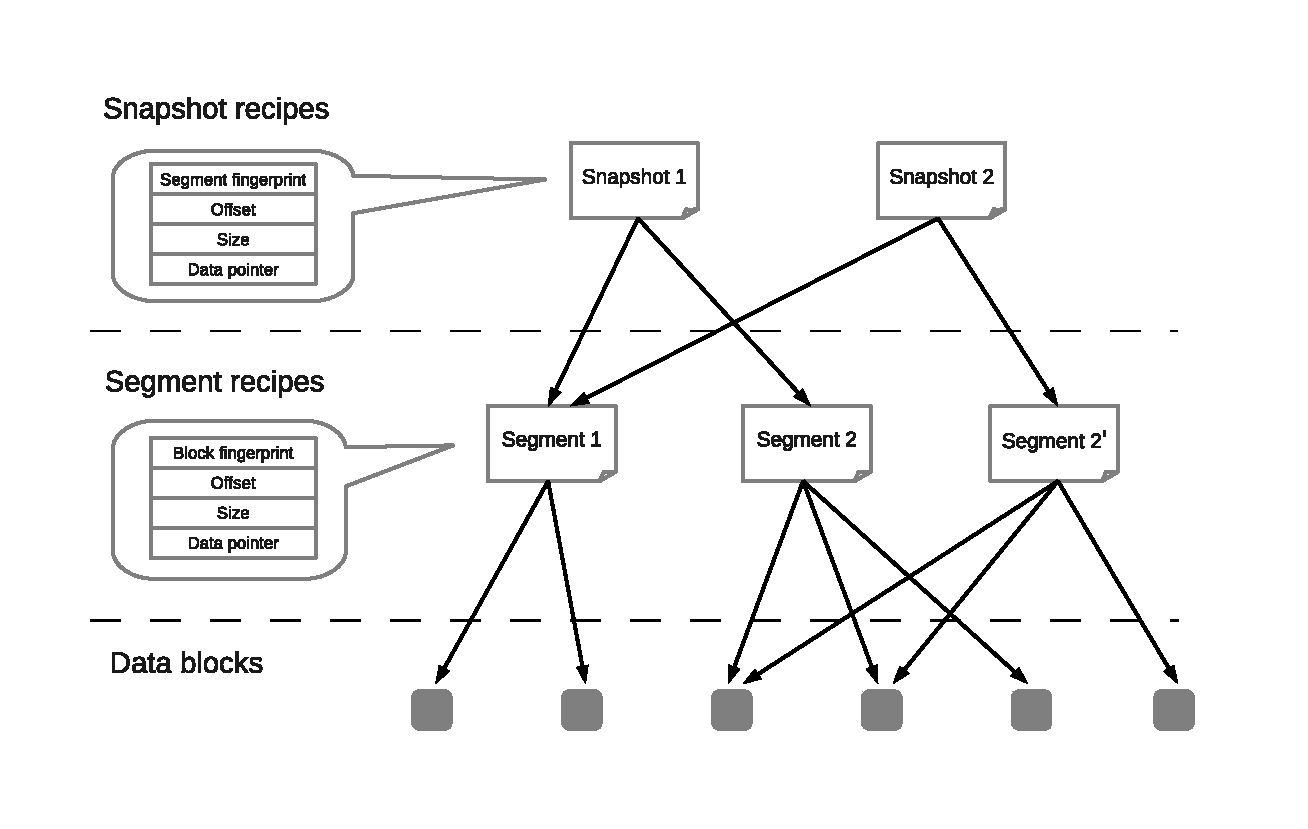
\epsfig{file=images/snapshot_representation.eps, width=3.7in}
%  \caption{An example of snapshot representation.}
%  \label{fig:snapshot}
%\end{figure}
%We choose this two-level structure because in practice we
%observe that during each backup period only a small amount of VM data are added or modified. 
%As the result, even the metadata of two snapshots can be highly similar, 
%thus aggregating a large number of chunks as one segment can significantly reduce the space cost of snapshot metadata.
%Furthermore, instead of using variables-sized segments, we use a dirty bit to capture the change status of fix-sized
%segments which greatly ease the segment-level deduplication.

In both two kind of recipes, 
they do not include the actual data but only have
 references pointers to the data which are either stored in backup storage or CDS.
In our implementation the data reference is a 8 bytes field which is either an 
ASID (discuss in \ref{sect:append} or an offset of 
An additional flag indicates


The architecture of our snapshot backup service contains the following components:
\begin{itemize}

\item  The backup storage layer. 
That stores snapshots on a distribued file system. 
Our prototype implementtion uses the QFS.
Since the distributed file system such as Hadoop and GFS takes the large block size such as 64MB,
and the data blcok size for dueduplication is nonuniform with 4KB on average,
we have added a layer to accmulate  data blocks from the deduplicated stream, and 
package them as 64MB, and apply data compression when applicable.

\item The deduplication layer.

\end{itemize}

Our architecture is built on the Aliyun platform which provides the largest public VM cloud in China. 
A typical VM cluster in our cloud environment
consists of from hundreds to thousands of physical machines, each of which can
host tens of xen-based\cite{Barham2003} VMs.

Aliyun has built a hadoop-like platform, which includes
several highly scalable cloud infrastructure services to support
 runing large scale VM cloud service:
\begin{itemize}
\item \textbf{DFS}: a distributed file system that is optimized for many large and sequential reads or appends.
%\item \textbf{KV}: a distributed key-value store for managing structured data.
\item \textbf{MapReduce}: a distributed data processing framework supports Map-Reduce\cite{Dean2004}.
\item \textbf{MemCache}: a distributed memory object caching system.
\end{itemize}
Our snapshot system and the virtual machine management service rely on these basic cloud services
to be functional:
DFS holds the responsibility of managing physical disk storage
in the cloud, all data needed for VM services, such as virtual disk images used by runtime VMs,
and snapshot data for backup purposes, reside in this distributed file system. 
In addition, our snapshot system 
places the index of CDS in MemCache for deduplication, 
and uses MapReduce to facilitate the offline
data processing. All the above services can easily find their open-source counterparts,
which shows the generality of our architecture and deduplication scheme.

User control VMs through the virtual machine management service.
During VM creation, a user chooses a pre-configured VM image or
a snapshot that contains an OS,
then the VM management service 
copies the corresponding VM image to her VM as the OS disk.
Data disks can be created and mounted onto the VM in the same way,
either empty or from an existing snapshot. 
All these virtual disks are represented as virtual disk image files in our
underline runtime VM storage system.  
To avoid network latency and congestion, 
our distributed file system place the primary replica of VM's 
image files at physical machine of VM instance.
When user deletes her VM, all the runtime virtual disk images and
their snapshot data are removed from DFS.

%ss operations
In each VM, 
the runtime I/O between virtual machine and its virtual
disks is tunneled by the virtual device driver (called TapDisk\cite{Warfield2005} at Xen).
This is also where our snapshot system is built in. Three major snapshot operations are supported:
\begin{itemize}
\item \textit{Write snapshot}: save the current state of virtual disk as a snapshot.
This is also where data deduplication would take place.
During snapshot backup, concurrent disk write is logged 
to ensure a consistent snapshot version is captured. 
\item \textit{Read snapshot}: restore the state of virtual disk from a snapshot.
\item \textit{Delete snapshot}: delete a snapshot and reclaim the disk space for unused data.
\end{itemize}

\begin{figure}[htbp]
  \centering
  %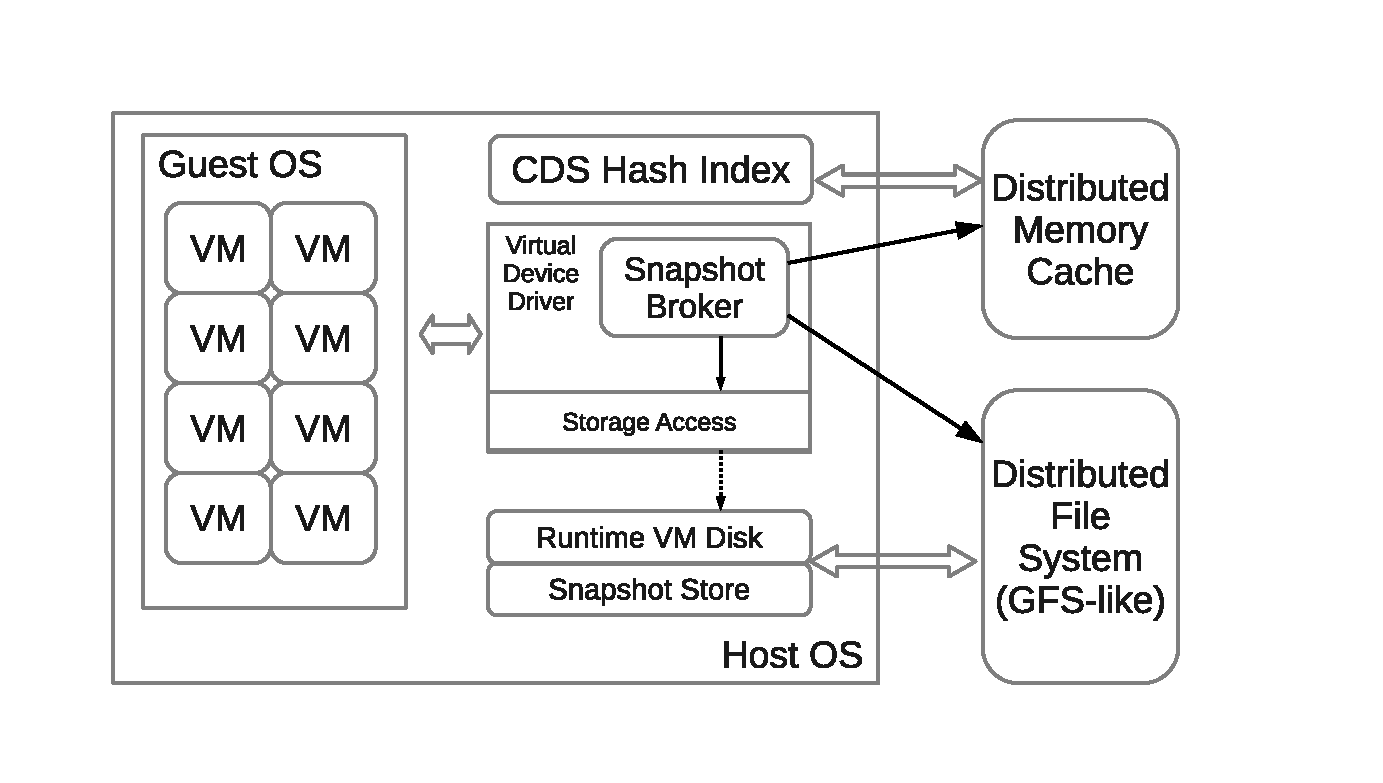
\epsfig{file=images/arch.eps, height=2in, width=2.66in}
  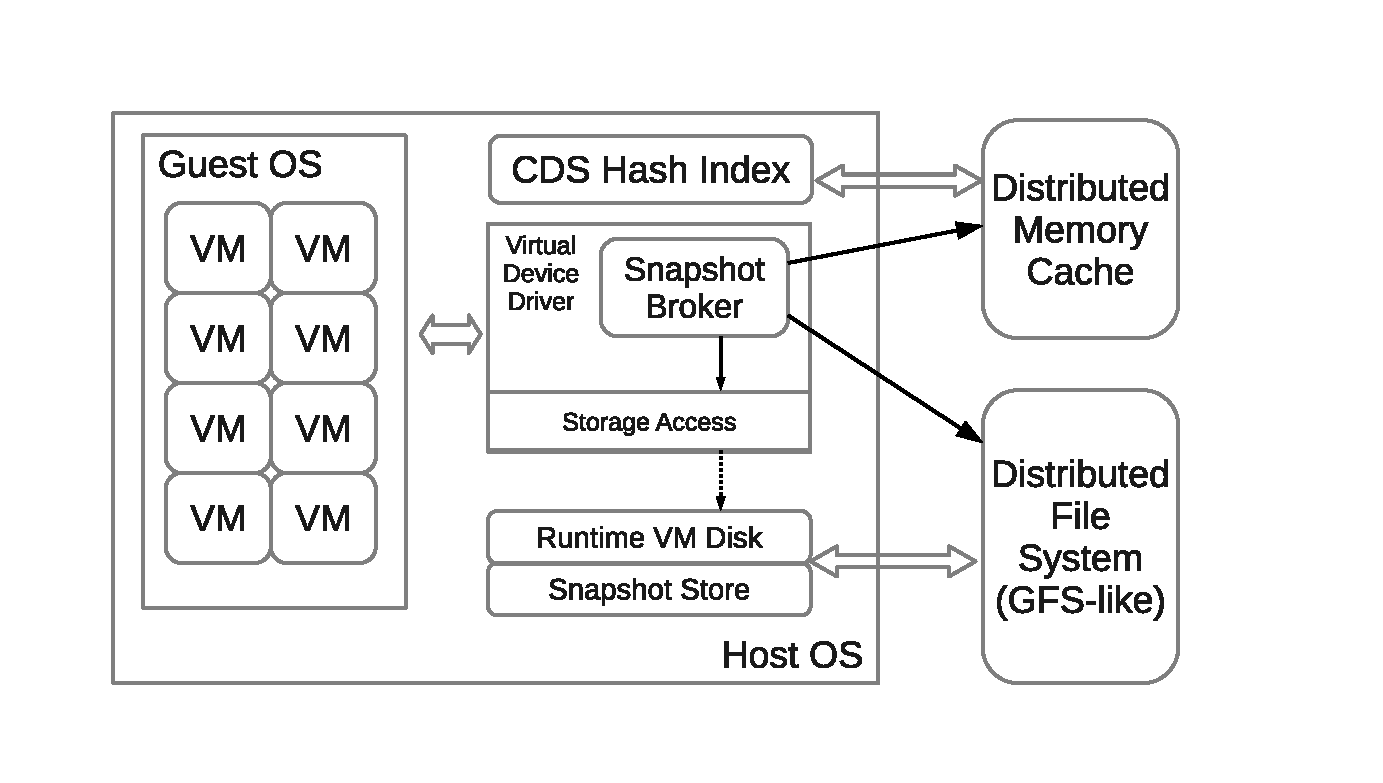
\epsfig{file=images/arch.eps, width=3.9in}
  \caption{Snapshot backup architecture of each node.}
  \label{fig:arch}
\end{figure}

Figure~\ref{fig:arch} shows the architecture view of our snapshot service
at each node. The snapshot broker provides the functional interface for  snapshot backup, access, and deletion.
The inner-VM  deduplication is conducted by the broker to access meta data in the snapshot data store
and we discuss this in details in Section~\ref{sect:innerVM}.
The cross-VM deduplication is conducted by the broker to access 
a common data set (CDS) (will discuss in Section~\ref{sect:crossVM},
whose block hash index is stored in a distributed memory cache. 

%\section{Multi-level Snapshot Deduplication}
\label{sect:dedupe}

\subsection{Snapshot System}
%system arch
Our architecture is built on the Aliyun platform which provides the largest public VM cloud in China. 
A typical VM cluster in our cloud environment
consists of from hundreds to thousands of physical machines, each of which can
host tens of xen-based\cite{Barham2003} VMs.

Aliyun has built a hadoop-like platform, which includes
several highly scalable cloud infrastructure services to support
 runing large scale VM cloud service:
\begin{itemize}
\item \textbf{DFS}: a distributed file system that is optimized for many large and sequential reads or appends.
\item \textbf{KV}: a distributed key-value store for managing structured data.
\item \textbf{MP}: a distributed data processing framework which is similar to Map-Reduce\cite{Dean2004}.
\item \textbf{MemCache}: a distributed memory object caching system.
\end{itemize}
%GFS-like\cite{googlefs03} 
%BigTable-like\cite{Chang2008a} 
Our snapshot system and the virtual machine management service rely on these basic cloud services
to be functional:
DFS holds the responsibility of managing physical disk storage
in the cloud, all data needed for VM services, such as virtual disk images used by runtime VMs,
and snapshot data for backup purposes, reside in this distributed file system. 
In addition, our snapshot system 
places the index of CDS in MemCache for deduplication, 
stores small amount of snapshot metadata in KV, and uses FX to facilitate the offline
data processing. All the above services can easily find their open-source counterparts,
which shows the generality of our architecture and deduplication scheme.

User control VMs through the virtual machine management service.
During VM creation, a user chooses a pre-configured VM image or
a snapshot that contains an OS,
then the VM management service 
copies the corresponding VM image to her VM as the OS disk.
Data disks can be created and mounted onto the VM in the same way,
either empty or from an existing snapshot. 
All these virtual disks are represented as virtual disk image files in our
underline runtime VM storage system.  
To avoid network latency and congestion, 
our distributed file system place the primary replica of VM's 
image files at physical machine of VM instance.
When user deletes her VM, all the runtime virtual disk images and
their snapshot data are removed from DFS.

%ss operations
In each VM, 
the runtime I/O between virtual machine and its virtual
disks is tunneled by the virtual device driver (called TapDisk\cite{Warfield2005} at Xen).
This is also where our snapshot system is built in. Three major snapshot operations are supported:
\begin{itemize}
\item \textit{Write snapshot}: save the current state of virtual disk as a snapshot.
This is also where data deduplication would take place.
During snapshot backup, concurrent disk write is logged 
to ensure a consistent snapshot version is captured. 
\item \textit{Read snapshot}: restore the state of virtual disk from a snapshot.
\item \textit{Delete snapshot}: delete a snapshot and reclaim the disk space for unused data.
\end{itemize}

\begin{figure}[htbp]
  \centering
  %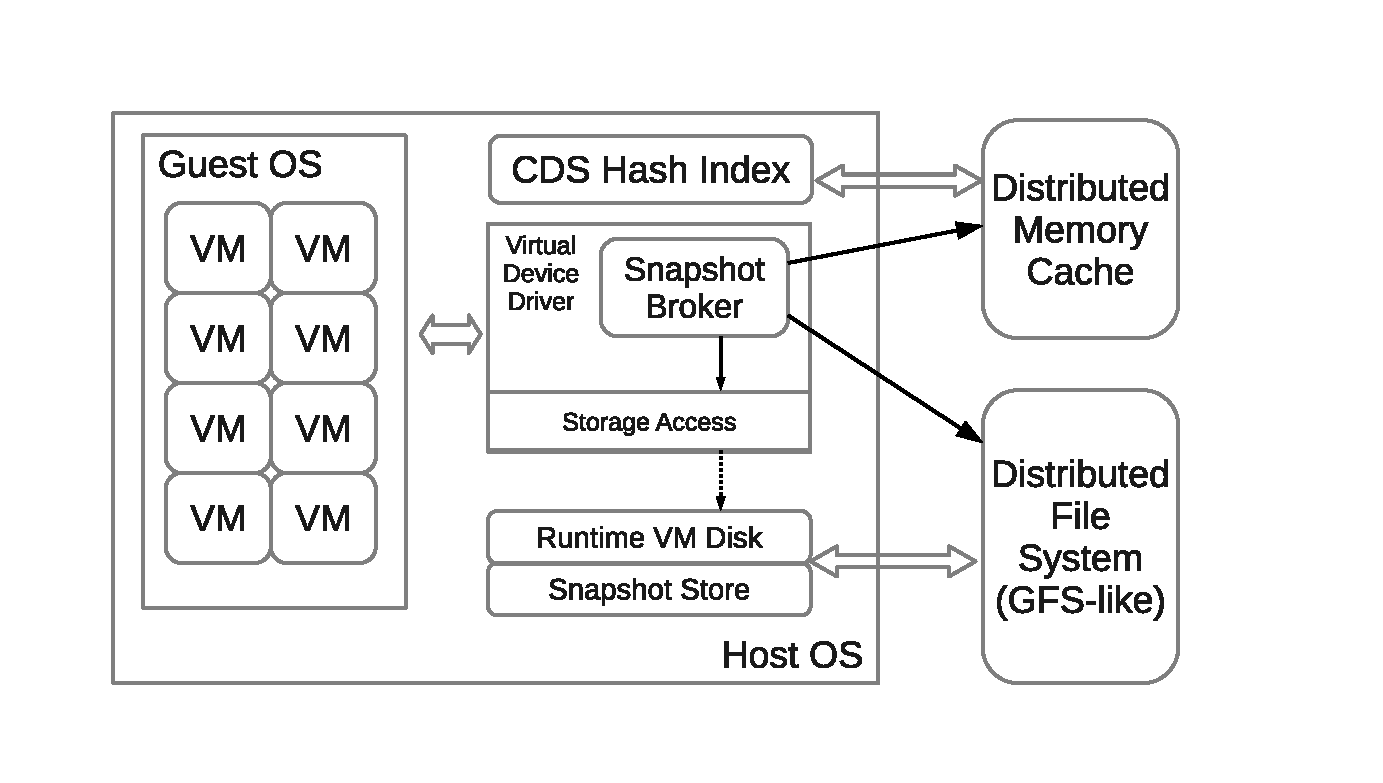
\epsfig{file=images/arch.eps, height=2in, width=2.66in}
  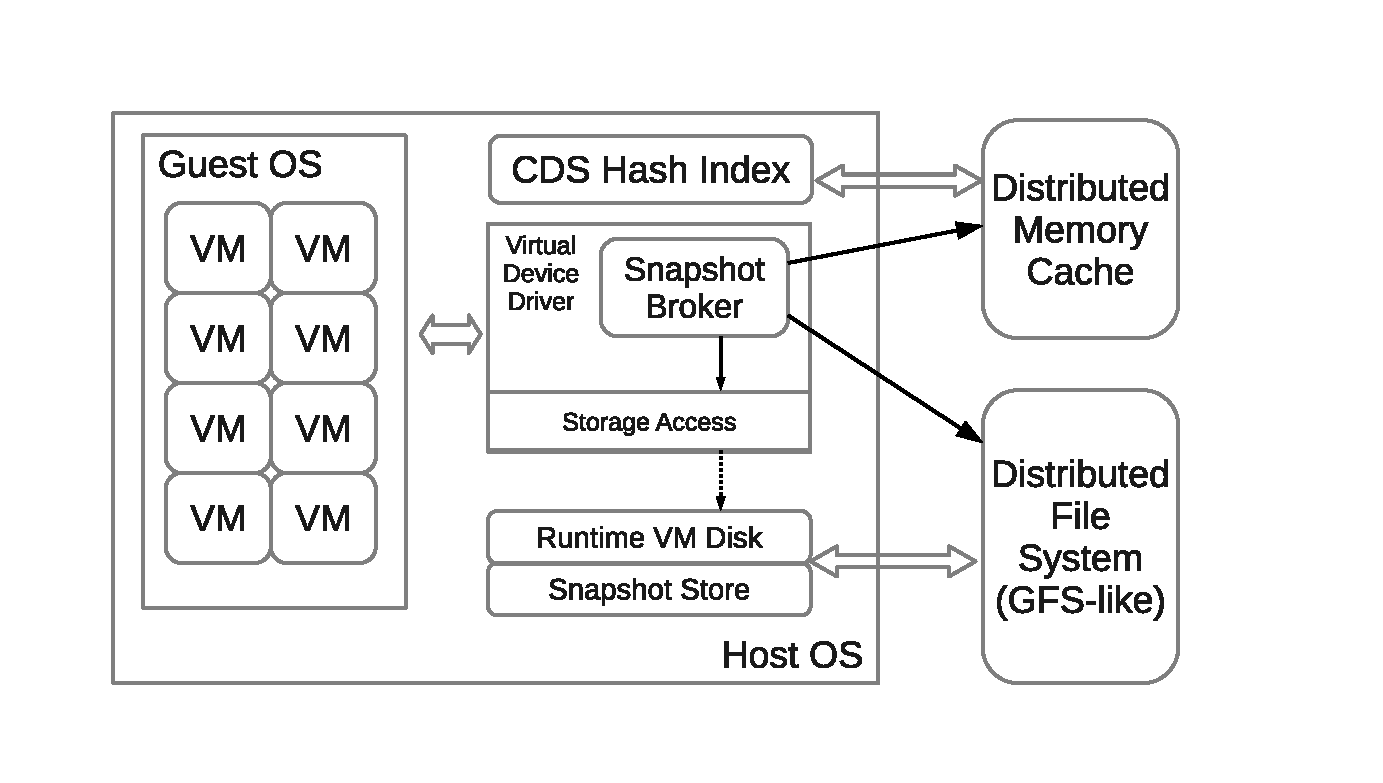
\epsfig{file=images/arch.eps, width=3.9in}
  \caption{Snapshot backup architecture of each node.}
  \label{fig:arch}
\end{figure}

Figure~\ref{fig:arch} shows the architecture view of our snapshot service
at each node. The snapshot broker provides the functional interface for  snapshot backup, access, and deletion.
The inner-VM  deduplication is conducted by the broker to access meta data in the snapshot data store
and we discuss this in details in Section~\ref{sect:innerVM}.
The cross-VM deduplication is conducted by the broker to access 
a common data set (CDS) (will discuss in Section~\ref{sect:crossVM},
whose block hash index is stored in a distributed memory cache. 

%snapshot representation
\subsection{Snapshot Representation}
The virtual device driver uses a bitmap to track the changes 
that have been made to virtual disk.
Every bit in the bitmap represents a fix-sized (2MB) region called \textit{segment}, indicates whether the segment
is modified since last backup. Hence we could treat segment as the basic unit in snapshot backup similar to
file in normal backup: a snapshot could share a segment with previous snapshot it is not changed. 
Moreover, we break 
segments into var-sized chunks (average 4KB) using content-based chunking algorithm,
which brings the opportunity of fine-grained deduplication by
allowing data sharing between segments.

\begin{figure}[htbp]
  \centering
  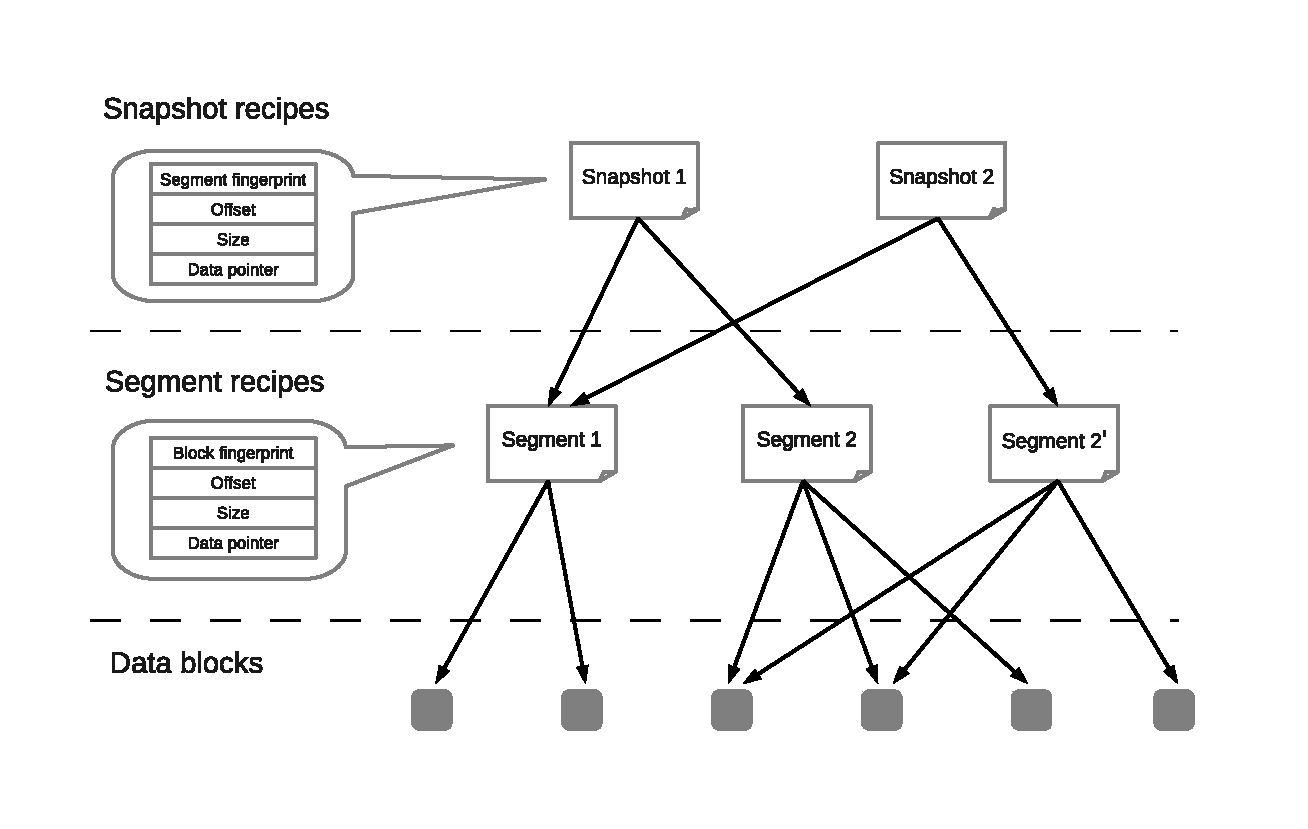
\epsfig{file=images/snapshot_representation.eps, width=3.7in}
  \caption{An example of snapshot representation.}
  \label{fig:snapshot}
\end{figure}
As a result, the representation of each snapshot is designed as a two-level index data structure 
in the form of a hierarchical directed acyclic graph as shown in Figure \ref{fig:snapshot}.
A snapshot recipe contains a list of segments, each of which is represented as a segment recipe
that holds the meatdata of its chunks. We choose this two-level structure because in practice we
observe that during each backup period only a small amount of VM data are added or modified. 
As the result, even the metadata of two snapshots can be highly similar, 
thus aggregating a large number of chunks as one segment can significantly reduce the space cost of snapshot metadata.
Furthermore, instead of using variables-sized segments, we use a dirty bit to capture the change status of fix-sized
segments which greatly ease the segment-level deduplication.

In both two kind of recipes, 
they do not include the actual data but only have
 references point to the data which are either stored in append store or CDS.
In our implementation the data reference is a 8 bytes field which is either an 
ASID (discuss in \ref{sect:append} or an offset of 
An additional flag indicates

\subsection{Multi-level Deduplication}
The multi-level deduplication scheme is designed base on the observations on the VM snapshot data from production cloud.
We found snapshot data duplication can be easily classified into two categories: \textit{Inner-VM} and \textit{Cross-VM}. 
Inner-VM duplication exists between VM's snapshots, because the majority of data are unchanged during each backup period. 
On the other hand, Cross-VM duplication is mainly due to widely-used software and libraries such as Linux and MySQL. 
As the result, different VMs tend to backup large amount of highly similar data.
Our multi-level pipeline process can minimize the cost of deduplication while maximize the its efficiency at each level,
and it is highly parallelizable since each segment is processed independently.

\subsubsection{Inner-VM Deduplication}
\label{sect:InnerVM}
The first-level deduplication is logically localized within each VM.
Such localization increases data independency between different VM backups,
simplifies snapshot management and statistics collection,
and facilitates parallel execution of snapshot operations.

The inner VM deduplication contains two levels of duplicate detection efforts:
\begin{itemize}
\item \textit{Level 1 Segment modification detection}.
If a segment is not changed, then its segment recipe can be simply reused by copying the data
reference from previous snapshot recipe. 
\item \textit{Level 2  Chunk fingerprint comparison.}
If a segment is modified, we perform fine-grained deduplication 
by comparing the fingerprints of its chunks to the same segment's recipe in the previous snapshot,
thus eliminate partial data duplication within the segment.
\end{itemize}

In general, operations at level 1 have almost no cost and most of unmodified data are filtered here. 
To process a dirty segment at level 2, 
there requires no more than one DFS access to load the segment recipe from previous snapshot,
and a tiny amount of memory to hold it in main memory.
\textit{may need details here}

\subsubsection{Cross-VM Deduplication}
\label{sect:CrossVM}

\subsection{Common Data Set}
%arch
%analysis
\section{Append Store}
\label{sect:append}
\subsection{Introduction}
Append Store (AS) is our underlining storage engine for storing snapshot data after deduplication. 
AS is built on top of our highly scalable distributed file system (DFS), 
which is very similar to Google's file system
in a sense that it is optimized for large files and sequential read/append operations.

\subsection{Design considerations}
While scalability has been handled by the DFS, there are still several challenges in 
storing billions of var-sized small data chunks:
\begin{description}
\item[Locality perseveration] Chunk data must be placed next to each other in the order of their writing sequence,
because reading a snapshot incurs large sequential reads of chunks under their logical sequence in the snapshot.
\item[Flexible referencing] To avoid overwhelming metadata operation capbility of DFS's master, 
we have to group small chunks into large data files in DFS.
However, snapshot deletion brings chunk data deletion, and reclaiming disk space would require many chunk data being moved.
If such chunk movement incurs updates of data referencing in snapshot and segment recipes, then the cost of deleting 
a snapshot would be extremely high.
\item[Efficient chunk lookup] The translation from data reference to data location must be very efficient in two ways: 
first, a sorted index is necessary to fast locate the data location in $O(log(n)$ time; 
second, the size of index must be optimized to minimized its memory footprint and the cost of fetching index. 
\end{description}



\subsection{Architecture}
\begin{figure}[htbp]
  \centering
  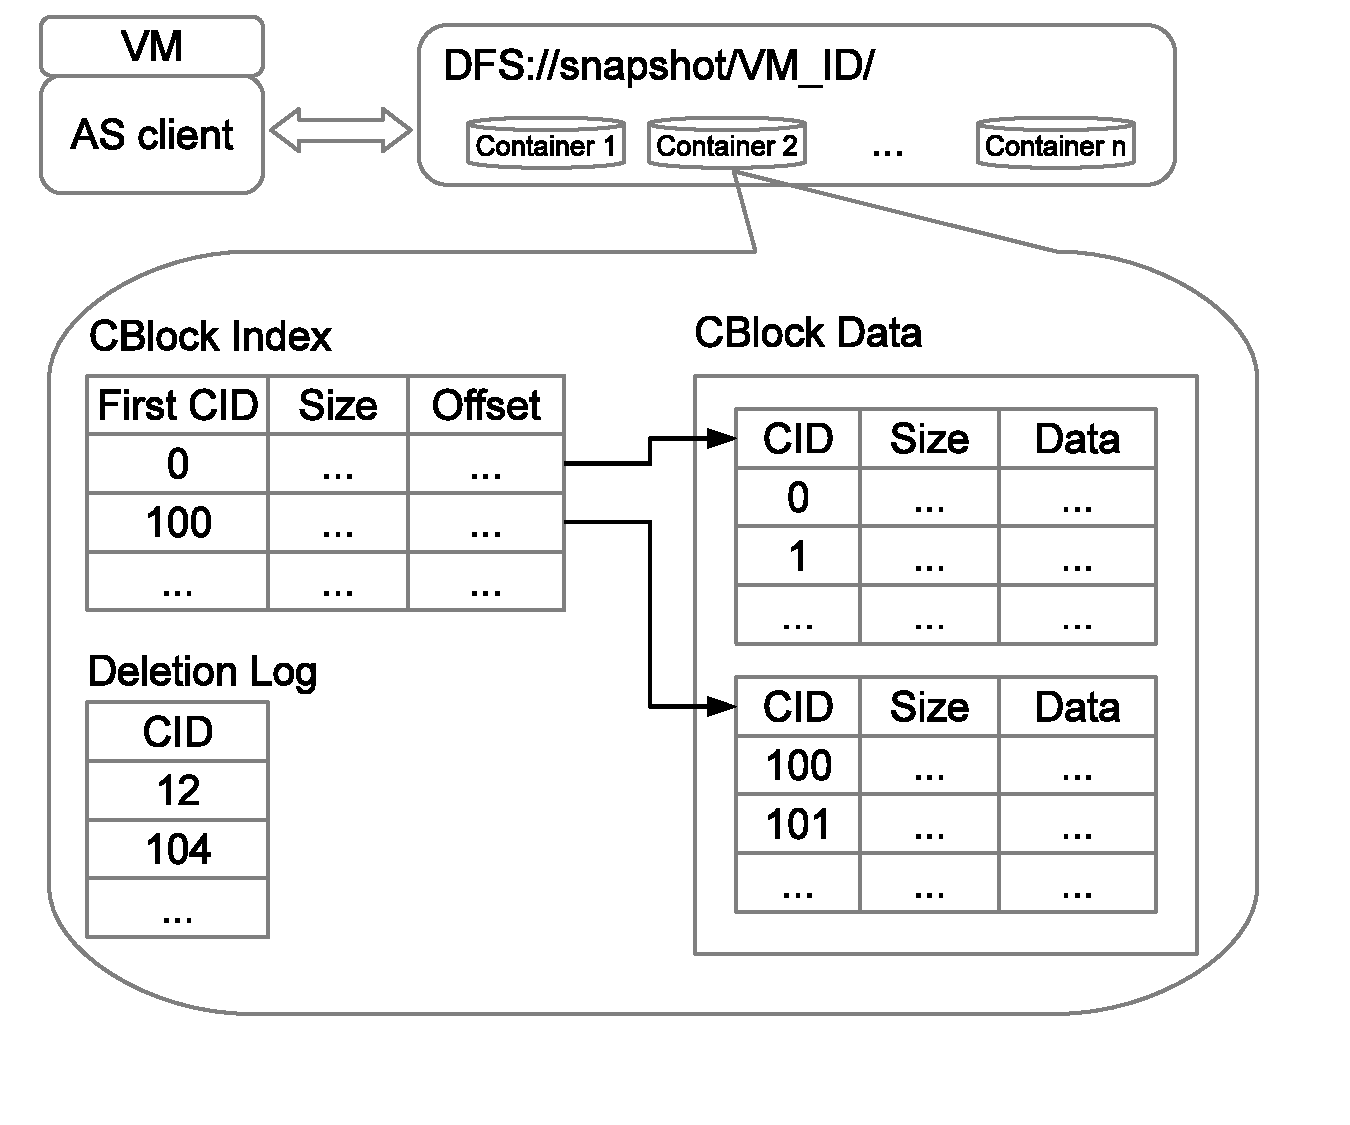
\epsfig{file=images/append_store_arch.pdf, width=3.5in}
  \caption{Architecture of Append Store}
  \label{fig:as_arch}
\end{figure}

Append Store supplies three interfaces: {\em get(ref)} accepts a data reference and retrives data, 
{\em put(data)} accepts data and returns a reference to be stored in metadata recipes, 
{\em delete(ref)} 
deletes the data pointed by the reference.
Under the hood, small var-sized data are grouped and stored into larger data containers. Each VM has
its snapshot data stored in its own Append Store, specified by the VM ID. 
We split every Append Store into multiple data containers so that reclaiming the disk space would not 
result in rewriting all the data at the same time.

As shown in Fig.\ref{fig:as_arch}, every data container is represented as three data files in DFS:
the data file holds all the actual data, the index file is responsible for translating data reference
into data locations, and a deletion log file remembers all the deletion requests to the container.

A data reference is composed of two parts: a container ID (2 bytes) and CID (6 bytes).
Append Store assign every piece of data a CID for its internal data referencing. 
When new data is appended, its CID is the current largest CID in that container plus one.
As a result, all the data locations are naturally indexed by this self-incremental CID, 
no extra sorting is needed.

Append Store groups multiple chunk data (i.e., 100) into larger units, called {\em CBlock}.
CBlock is the basic unit for append store's internal read/write/compression.
There is one index entry in the container index corresponding to every CBlock. It keeps the first chunk's CID
in that CBlock, and the CBlock data's size and location.

Using CBlock brings us several advantages: First, the write workload to DFS master is greatly reduced; second, grouping
small chunks gives better compression. Third, reading a CBlock (200 - 600 KB) typically cost the same amount of disk 
seek as reading a 4KB chunk. Finally, this greatly reduces the size of index. Let $m$ be the number of chunks in each
CBlock, then the overall index size is reduced to $1/m$. In our implementation, using $m=100$ reduces the index for
a 1GB container from 10 MB to 100 KB.

\subsection{Operations}
In order to read a chunk data by reference, Append Store client first loads the
container index file specified by the container ID, then search the CBlock index to find the entry that covers the chunk by CID.
After that, it reads the whole CBlock data from DFS, decompress it, seek the exact chunk data specified by CID. 
Finally, the client updates itws internal chunk data cache with the newly loaded contents to anticipate future sequential reads.

Write requests to append store are accumlated. When the number reaches $m$, the AS client forms a CBlock by assigning 
every chunk a CID, compress the CBlock data, and append it to the CBlock data file. Then a new CBlock index entry is appended
to CBlock index.

Append store adopts lazy delete strategy. The deletion requests are appended into every container's deletion log file with the CID of data to be deleted.
CIDs in deletion log are guaranteed to be referenced by nobody and can be safe deleted in future. 
Periodically, snapshot management system asks append store to compact containers in order to reclaim disk space. 
The actual compaction will only take place when the number of deleted items reached $d\%$ of container's capacity. 
During compaction, append store creates a new container (with the same container ID) to replace the 
existing one. This is done by sequentially scan the old container, copying all the chunks that are not 
found in deletion log to the new container, creating new CBlocks and indices. 
However, every chunk's CID is plainly copied rather than re-generated. This does not affect the sorted
order of CIDs in new container, but just leaving holes in CID values. As the result, all data references stored 
in upper level recipes are unaffected, and the data reading process is as efficient as before.

%hard problems

\subsection{Analysis}

Snapshot operation performance analysis:
\begin{table}
    \begin{tabular}{l p{1.5in} l}
        \hline
        Symbol & Description & Measurement \\ \hline
        $N_{seg}$ & Number of segments in the snapshot & ~ \\ [1ex] \\ [-1.5ex]
        $N_{chunk}$ & Number of chunks in one segment & ~ \\ [1ex] \\ [-1.5ex]
        $P_{dirty}$ & Probablity of a segment is dirty & ~ \\ [1ex] \\ [-1.5ex]
        $P_{new}$ & Percentage of new data & ~ \\ [1ex] \\ [-1.5ex]
        $P_{change}$ & Probablity that a chunk is not found in parent snapshot & ~ \\ [1ex] \\ [-1.5ex]
        $P_{in\_CDS}$ & Percentage of chunks in CDS & ~ \\ [1ex] \\ [-1.5ex]
        $T_{scan}$ & Time to scan segment data and caculate content hash & 74 ms \\ [1ex] \\ [-1.5ex]
        $T_{write\_AS}$ & Time of writing a chunk into append store & 0.24 ms \\ [1ex] \\ [-1.5ex]
        $T_{read\_AS}$ & Time of reading a chunk from append store & ~ \\ [1ex] \\ [-1.5ex]
        $T_{read\_chunk}$ & Time of reading a chunk & ~ \\ [1ex] \\ [-1.5ex]
        $T_{check\_CDS}$ & Time of checking CDS & ~ \\ [1ex] \\ [-1.5ex]
        $T_{read\_CDS}$ & Time of reading a chunk data from CDS data store& ~ \\
        \hline
    \end{tabular}
    \caption{List of performance factors}
    \label{tab:as_param}
\end{table}

The overall time of writing a snapshot is:

\begin{dmath}
T_{write} = P_{dirty} * N_{seg} * [max(T_{scan}, T_{read\_AS}) + P_{change} * N_{chunk} * T_{check\_CDS} + P_{new} * N_{chunk} * T_{write\_AS}]
\end{dmath}

The overall time to read a snapshot is:

\begin{dmath}
T_{read} = N_{seg} * {T_{read\_AS} + N_{chunks} * [P_{in\_CDS} * T_{read_CDS} + (1 - P_{in\_CDS}) * T_{read\_chunk}]}
\end{dmath}

Average time of reading a chunk:

\begin{dmath}
T_{read\_chunk} = P_{in\_CDS} * T_{read\_CDS} + (1 - P_{in\_CDS}) * T_{read\_AS}
\end{dmath}

Time of reading append store:

\begin{dmath}
T_{read\_AS} = 0 * P_{in\_cache} + (1 - P_{in\_cache} ) * T_{load\_CBlock}
\end{dmath}

\section{Deletion}
In a mature VM cluster, snapshot deletions are as frequent as snapshot creations.
Our system adopts lazy delete strategy so that all snapshot deletions are scheduled
in the backup time window at midnight. 
Therefore, snapshot deletions must be fast enough to fit in time window and
efficient enough to satisfy our resource constraints.
However, there is no simple solution can achieve these goals with high reliability.
In Aliyun's cloud, we use a {\em fuzzy deletion} method to trade deletion accuracy for
speed and resource usage. This method tolerates a tiny percentage of storage leakage
to make the deletion operation faster and efficient by an order of magnitude,
yet we still adopt an slow but accurate deletion method to fix such leakage in the long-term.
Our hybrid deletion strategy, using fuzzy deletion regularly and accurate deletion periodically,
accomplishs our speed, resource usage and relibility goals very well.

% \subsection{Challenges}
% Contrary to a traditional backup system, a dedupe system shares data among files by default. 
% Reference management is necessary to keep track of chunk usage and reclaim freed space. 
% In addition to scalability and speed, reliability is another challenge for reference management. 
% If a chunk gets freed while it is still referenced by snapshots, data loss occurs and files cannot be restored. 
% On the other hand, if a chunk is referenced when it is actually no longer in use, it causes storage leakage.

% Reference counting, while being simple, suffers from low reliability especially in our distributed environment, 
% because it is vulnerable to lost or repeated updates: when errors occur some chunks maybe updated and some may not. 
% Complicated transaction rollback logic is required to make reference counts consistent. Moreover, 
% there is almost no way to verify if the reference count is correct or not in a large dynamic system. 
% In real deployments, where data integrity and recoverability directly affect product reputation, simple reference counting is unsatisfactory.

% Mark-and-sweep is generally a better solution. During the mark phase, all snapshot recipes are traversed so as to mark the used chunks. 
% In the sweep phase all chunks are swept and unmarked chunks are reclaimed. 
% This approach is very resilient to errors: at any time the process can simply be restarted with no negative side effects. 
% Scalability, however, is an issue. {\em needs to explain its resource usage}


\subsection{Approximate Deletion}
\begin{figure}[htbp]
  \centering
  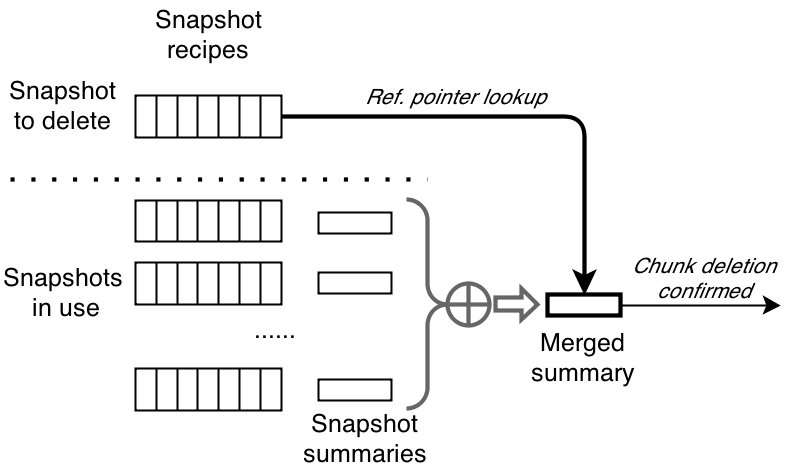
\epsfig{file=images/deletion.png, width=3.5in}
  \caption{Approximate deletion}
  \label{fig:deletion_flow}
\end{figure}

We design approximate deletion to fast identify unused data in the append store.
Instead of scanning the whold append store, it uses a bloom filter to check 
if a data are still referenced by living snapshots. However, there is a small false-positive probility which
would indetify unused data as in use, i.e., storage leakage.
The following steps would take place during an approximate deletion:

\begin{enumerate}
\item {\bf Creating bloom filter} Scan all the living snapshot recipess and their segment recipes,
for every reference pointing to append store, add it to the bloom filter.
\item {\bf Check existance} For every data reference in the deleted snapshot recipe and its segment recipes,
check the existance of that data reference in bloom filter. If not found, it is safe to delete that piece of data from append store
because no living snapshots has referenced it.
\end{enumerate}

The overall time of running a approximate deletion for one snapshot deletion would be scanning
all the living snapshots and deleted snapshots, since operations on the in-memory bloom filter can be done in
parallel and is much faster than loading recipes from DFS:
\begin{equation}
T = (N_{SS} + 1) * T_{scan\_recipes}
\end{equation}
 
Using the example and analysis in previous section, this approximate deletion can be done in 5 minutes. 
Memory usage of the bloom filter depends on its false-positive probility $P_{bl}$,
when set $P_{bl}$ to 0.01, the memory footprint of approximate deletion is about 15 MB.

The design goal of approximate deletion is to reduce the frequency of running accurate deletion.
For one VM's snapshots, let $D_{leakage}$ be the amount of storage leakage, $D_{del}$ be the average amount of data
to be deleted in one snapshot deletion, 
then we have:
\begin{equation}
D_{leakage} = N_{approximate} * P_{bl} * D_{del}
\end{equation}
where $N_{approximate}$ is the number of runs of approximate deletion. 
An accurate deletion is triggered to fix the storage leakage
when $D_{leakage}/D_{del}$ is accmulated to exceed certain threshold $T$:
\begin{equation}
D_{leakage} / D_{del} = N_{approximate} * P_{bl} > T \Rightarrow N_{approximate} > T/P_{bl}
\end{equation}
Therefore, when $P_{bl} = 0.01$ and $T=1$, 
there would be a run of accurate deletion for every $T/P_{bl} = 100$ runs of approximate deletion.
On a machine that hosts 20 VMs and each VM deletes snapshot daily, there would be less than
one accurate deletion scheduled per day.

\subsection{Accurate Deletion}
Our accurate deletion uses mark-and-sweep to find all the unused chunks in a VM's append store.
The following steps would take place during an accurate deletion:

\begin{enumerate}
\item Scan all the containers. For each container, extract full list of existing data references and allocate a bitmap. 
(Notice this list is self sorted.)
\item Scan all the snapshot recipes and segment recipes. For every data reference pointing to append store,
find it in the above lists and mark the corresponding position in bitmaps.
\item Scan the bitmaps, for every bit that are not marked, tell append store the corresponding data reference can be deleted.
\end{enumerate}

Although accurate deletion guarantees reliability and correctness, its speed and resource usage are big problems to our VM cloud.
Let $T_{scan\_AS}$ be the time to scan the VM's append store, $T_{scan\_recipes}$ be the time to scan one snapshot recipe
and its segment recipes, $T_{mark}$ be the time of finding a data reference in the list and mark bitmap, 
$N_{SS}$ be the number of snapshots and $N_c$ be the number of chunks in one snapshot.
The overall time of running an accurate deletion for one VM is:
\begin{equation}
T = T_{scan\_AS} + N_{SS} * T_{scan\_recipes} + N_{SS} * N_c * T_{mark}
\end{equation}

For a virtual disk that has 10 snapshots, 50 GB of data in the append store, $T_{scan\_AS}$ would have cost half an hour already.
In addition, scanning recipes of 10 snapshots cost another 5 minutes.
Furthermore, maintaining the full lists of data references and bitmaps costs about 100 MB of memory. Having tens of VMs
co-lived in one physical machine and deleting snapshot on a daily basis, 
it's infeasible to run accurate deletion as frequent as snapshot deletions.

\subsection{Discussion}

